%%% Plantilla creada para Proyecto de Investigación
%%% Sistemas Inteligentes
%%% Rodrigo Barba Guamán
%%% lrbarba@utpl.edu.ec
%%% Ver 1.1, abril 2024

\documentclass[a4paper,12pt]{article}

\usepackage[utf8]{inputenc}
\usepackage[spanish]{babel}
\usepackage{amsmath}
\usepackage{amsfonts}
\usepackage{amssymb}

\usepackage{graphicx}
\usepackage{hyperref}
\usepackage{wrapfig}
\usepackage{enumitem}
\usepackage{fancyhdr}
\usepackage{float}
\usepackage{eurosym}
\usepackage{color}
\usepackage{titling}
\usepackage{lipsum}
\usepackage{tocbibind}
\usepackage{listings}
\usepackage{xcolor}

\usepackage[left=3cm,right=3cm,top=3cm,bottom=4cm]{geometry}


\pagestyle{fancy}


%%% librerias cabeceras
\newcommand{\hsp}{\hspace{20pt}}
\newcommand{\HRule}{\rule{\linewidth}{0.5mm}}
\headheight=50pt
%%%
\newcommand{\vacio}{\textcolor{white}{holacaracola}}

%%% Enumeración de ecuaciones
%%% con el número de sección y el de ecuación.
\renewcommand{\theequation}{\thesection.\arabic{equation}}


% Color azul para algunos
% textos de la portada
\definecolor{azulportada}{rgb}{0.16, 0.32, 0.75}

%%%% Azul para textos de headings
\definecolor{azulinterior}{rgb}{0.0, 0.2, 0.6}

% Configuración de listings para código Python
\definecolor{codegreen}{rgb}{0,0.6,0}
\definecolor{codegray}{rgb}{0.5,0.5,0.5}
\definecolor{codepurple}{rgb}{0.58,0,0.82}
\definecolor{backcolour}{rgb}{0.95,0.95,0.92}

\lstdefinestyle{pythonstyle}{
    backgroundcolor=\color{backcolour},
    commentstyle=\color{codegreen},
    keywordstyle=\color{magenta},
    numberstyle=\tiny\color{codegray},
    stringstyle=\color{codepurple},
    basicstyle=\ttfamily\footnotesize,
    breakatwhitespace=false,
    breaklines=true,
    captionpos=b,
    keepspaces=true,
    numbers=left,
    numbersep=5pt,
    showspaces=false,
    showstringspaces=false,
    showtabs=false,
    tabsize=2,
    language=Python
}

\lstset{style=pythonstyle}

%%%%%%%%%%%%%%%%%%%%%%%%%%%%%%%%
%%%%%% Datos del proyecto %%%%%%
%%%%%%%%%%%%%%%%%%%%%%%%%%%%%%%%
%%%TÍTULO
%%% Escribirlo en minúsculas, el programa
%%% lo pondrá en mayúsculas en la portada.
\title{Sistema de Reconocimiento Facial Basado en Aprendizaje Profundo}
%%%% AUTOR
\author{Luis Antonio Pillaga Zhagñay}
%%%%%%%%%%%%%%%%
%%%%%% DIRECTOR DEL TRABAJO
%%%%%%% Cambiar el nombre
\newcommand{\director}{Guido Eduardo Riofrío Calderón}
%%%%%%%%%%%%%%%

%%%%%%%%%%%%%%%%%%%%%
%%%%%%%%%%%%%%%%%%%%
\begin{document}

%%%%%%%%%%%%%%%%%%%%%%%%%%%%%%%
%%%%%%%%%%%%%%%%%%%%%%%%%%%%%%%
\begin{titlepage} %%%%% Aquí no hay que tocar nada.
	%%%% Las siguientes instrucciones generarán automáticamente
	%%%% la portada de tu proyecto.
	%%% Cambio de la estructura de esta página
\newgeometry{left=0.6cm,top=1.3cm,bottom=1.2cm}

\fbox{\parbox[c]{18.5cm}{
\begin{center}
\vspace{1.5cm}
{\fontfamily{phv}\fontsize{20}{6}\selectfont{Universidad Técnica Particular de Loja}}\\
[1em]
{\fontfamily{phv}\fontsize{16}{5}\selectfont{Métodos de Aprendizaje Profundo}}\\
[1em]
{\fontfamily{phv}\fontsize{26}{5}\selectfont{Maestría en Inteligencia Artificial Aplicada}}\\
[2.6cm]
% Autor del trabajo de investigación
\textcolor{azulportada}{\fontfamily{phv}\fontsize{16}{5}\selectfont{\theauthor}}\\
[1cm]
% Título del trabajo
\textcolor{azulportada}
{\fontfamily{phv}\fontsize{30}{5}\selectfont{\textsc{\thetitle}}}\\
%{\Huge\textbf{\thetitle}}\\
[1cm]
\includegraphics[width=3.5cm]{UTPL.png}
\\[2cm]
{\fontfamily{phv}\fontsize{16}{5}\selectfont{Docente}}\\
[0.5cm]
{\fontfamily{phv}\fontsize{16}{5}\selectfont{\director}}\\
[2cm]
{\fontfamily{phv}\fontsize{14}{5}\selectfont{octubre 2025 - febrero 2026}}\\
[4cm]
\end{center}
}}

 \restoregeometry
 %%%% Volvemos a la estructura de la página normal

\end{titlepage}

%%%%%%%%%%%%%%%%%%%%%%%%%%%%%%

{%\Large

\newpage

%%%Encabezamiento y pie de página
%%% También se genera automáticamente
%%% Mejor no tocarlo mucho.
\renewcommand{\headrulewidth}{0.5pt}
\fancyhead[R]{
	\textcolor{azulinterior}{\fontfamily{phv}\fontsize{14}{4}\selectfont{\textbf{\thetitle}}}\\
\textcolor{azulportada}{\fontfamily{phv}\fontsize{10}{3}\selectfont{octubre 2025 - febrero 2026}}\\
{\fontfamily{phv}\fontsize{10}{3}\selectfont{\theauthor}}}
\fancyhead[L]{\vacio}

\renewcommand{\footrulewidth}{0.5pt}
\fancyfoot[L]{\footnotesize Métodos de aprendizaje profundo}
\fancyfoot[C]{\vacio}
\fancyfoot[R]{\footnotesize Página \thepage}


%%%%%%%%%%%%%%%%%%%%

\

\vacio

\


\subsection*{Resumen}
El presente trabajo aborda el diseño e implementación de un sistema de reconocimiento facial orientado a la identificación de personas en tiempo real. Se desarrolló una arquitectura modular que integra técnicas modernas de detección de rostros mediante el modelo SCRFD, extracción de características faciales con ArcFace y búsqueda eficiente de vectores mediante FAISS. El sistema fue implementado en Python siguiendo principios de diseño orientado a objetos, lo que permite intercambiar componentes sin modificar la lógica central. Se realizaron pruebas de evaluación sobre un conjunto de imágenes de validación, obteniendo métricas de precisión que validan la efectividad del enfoque propuesto. Se incluye además una implementación alternativa basada en la biblioteca dlib y face\_recognition para fines comparativos y educativos.


\subsection*{Abstract}
\textsl{
This work addresses the design and implementation of a facial recognition system aimed at real-time person identification. A modular architecture was developed that integrates modern face detection techniques using the SCRFD model, facial feature extraction with ArcFace, and efficient vector search using FAISS. The system was implemented in Python following object-oriented design principles, allowing components to be swapped without modifying the core logic. Evaluation tests were conducted on a validation image set, obtaining precision metrics that validate the effectiveness of the proposed approach. An alternative implementation based on the dlib and face\_recognition libraries is also included for comparative and educational purposes.}

\ %% Así hago que se abra más espacio entre renglones.

\

\hrule

\

\


\paragraph{Palabras clave:} reconocimiento facial, aprendizaje profundo, ArcFace, FAISS, visión por computador.

\


\paragraph{Keywords:} facial recognition, deep learning, ArcFace, FAISS, computer vision.




\newpage

%%% En esta página va el índice,
%%% pero no hay que hacer nada porque
%%% se generará automáticamente.

\tableofcontents

\newpage



\section{Introducción}

Los avances en inteligencia artificial han transformado significativamente el campo del reconocimiento facial durante la última década. Lo que antes requería algoritmos manuales de extracción de características y clasificadores tradicionales, hoy se resuelve mediante redes neuronales profundas capaces de aprender representaciones discriminativas directamente de los datos \cite{wang2021}. Esta evolución ha posibilitado aplicaciones que van desde el desbloqueo de dispositivos móviles hasta sistemas de control de acceso en aeropuertos y edificios corporativos.

El reconocimiento facial presenta desafíos particulares que lo distinguen de otras tareas de visión por computador. A diferencia de la clasificación de objetos donde las categorías son fijas y conocidas, un sistema de reconocimiento facial debe ser capaz de identificar individuos específicos de un conjunto que puede cambiar dinámicamente. Además, debe manejar variaciones en pose, iluminación, expresión facial y oclusiones parciales, todo mientras mantiene tiempos de respuesta compatibles con aplicaciones en tiempo real \cite{deng2019}.

El presente proyecto surge de la necesidad de implementar un sistema funcional que permita comprender los fundamentos técnicos del reconocimiento facial moderno. Más allá de utilizar bibliotecas como cajas negras, se busca diseñar una arquitectura que exponga claramente cada etapa del pipeline: detección de rostros, alineación geométrica, extracción de embeddings y búsqueda por similitud. Esta transparencia resulta valiosa tanto para propósitos educativos como para futuras extensiones del sistema.


\subsection{\textbf{Objetivo general}}
\begin{itemize}
    \item Diseñar e implementar un sistema de reconocimiento facial basado en aprendizaje profundo que permita la identificación de personas en tiempo real mediante webcam o archivos de video.
\end{itemize}

\subsection{\textbf{Objetivos específicos}}
\begin{itemize}
    \item Investigar y analizar las técnicas actuales de detección facial y extracción de características basadas en redes neuronales profundas.
    \item Implementar una arquitectura modular que separe las responsabilidades de detección, alineación, embedding y matching.
    \item Desarrollar un proceso de enrolamiento que capture y almacene representaciones faciales de usuarios conocidos.
    \item Evaluar el rendimiento del sistema en términos de precisión de reconocimiento y velocidad de procesamiento.
    \item Comparar el enfoque basado en InsightFace/ArcFace con una implementación alternativa usando dlib/face\_recognition.
\end{itemize}

\section{Marco Teórico}

Esta sección presenta los fundamentos teóricos que sustentan el sistema desarrollado. Se describen las técnicas de detección facial, los métodos de extracción de características mediante redes profundas y los algoritmos de búsqueda vectorial empleados.

\subsection{Detección de Rostros}

La detección de rostros constituye la primera etapa de cualquier sistema de reconocimiento facial. Su objetivo es localizar las regiones de una imagen que contienen rostros humanos, típicamente mediante cajas delimitadoras (bounding boxes) y, opcionalmente, puntos de referencia faciales (landmarks).

\subsubsection{Histograma de Gradientes Orientados (HOG)}

El método HOG, propuesto originalmente para detección de peatones, ha sido ampliamente utilizado en detección facial \cite{king2017}. El algoritmo divide la imagen en celdas pequeñas y calcula histogramas de las direcciones de los gradientes dentro de cada celda. Estos histogramas locales se concatenan para formar un descriptor global que alimenta un clasificador SVM (Support Vector Machine).

La biblioteca dlib implementa un detector HOG frontal que opera eficientemente en CPU. Sus ventajas incluyen bajo consumo de recursos computacionales y robustez ante variaciones moderadas de iluminación. Sin embargo, presenta limitaciones en la detección de rostros con rotaciones significativas o de pequeño tamaño en la imagen.

\subsubsection{SCRFD: Sample and Computation Redistribution}

SCRFD representa el estado del arte en detectores faciales eficientes \cite{guo2021}. A diferencia de métodos anteriores que distribuyen uniformemente los recursos computacionales, SCRFD redistribuye tanto las muestras de entrenamiento como la capacidad del modelo hacia las escalas y regiones más relevantes para la detección.

El detector utiliza una arquitectura basada en Feature Pyramid Networks (FPN) con múltiples cabezas de predicción. Emplea Generalized Focal Loss para clasificación y DIoU loss para regresión de cajas. Además de las coordenadas de la caja delimitadora, SCRFD predice cinco puntos de referencia faciales (ojos, nariz, comisuras de la boca), esenciales para la posterior alineación.

Los experimentos reportados indican que SCRFD-34GF supera a TinaFace por 3.86\% en el conjunto difícil de WIDER FACE, siendo además tres veces más rápido en GPU \cite{guo2021}.

\subsection{Alineación Facial}

Una vez detectado un rostro, resulta necesario normalizarlo a una pose canónica antes de extraer características. Esta normalización compensa variaciones en la posición, escala y rotación del rostro dentro de la imagen.

La alineación funciona de manera similar a una foto de carnet: se busca que todos los rostros queden en la misma posición y tamaño. Para lograrlo, el sistema utiliza cinco puntos de referencia detectados en el rostro (los dos ojos, la punta de la nariz y las dos comisuras de la boca) y los desplaza a posiciones fijas predeterminadas.

El proceso consiste en:
\begin{enumerate}
    \item Detectar los 5 puntos de referencia en el rostro original
    \item Calcular una transformación geométrica que rota, escala y desplaza la imagen
    \item Aplicar esta transformación para obtener un rostro de 112$\times$112 píxeles perfectamente centrado
\end{enumerate}

El resultado es que sin importar si la persona estaba mirando ligeramente hacia un lado o si se encontraba más cerca o lejos de la cámara, el rostro alineado siempre tendrá los ojos, nariz y boca en las mismas coordenadas. Esto facilita enormemente la comparación posterior entre rostros.

\subsection{Extracción de Características: ArcFace}

La extracción de características faciales ha evolucionado desde descriptores manuales (LBP, Gabor) hacia representaciones aprendidas mediante redes neuronales convolucionales. El enfoque actual consiste en entrenar redes que proyecten imágenes faciales a un espacio de embeddings donde rostros de la misma persona queden cercanos y rostros de personas distintas queden alejados.

\subsubsection{El Concepto de Embedding Facial}

Un embedding facial puede entenderse como una ``huella digital numérica'' del rostro. La red neuronal toma una imagen de 112$\times$112 píxeles y la convierte en un vector de 512 números. Este vector captura las características únicas del rostro de forma compacta.

La idea clave es que dos fotos de la misma persona producirán vectores muy similares (apuntando en direcciones parecidas), mientras que fotos de personas diferentes producirán vectores distintos (apuntando en direcciones alejadas). Esta propiedad permite comparar rostros simplemente midiendo qué tan ``alineados'' están sus vectores.

\subsubsection{ArcFace: Mejorando la Separación entre Identidades}

ArcFace \cite{deng2019} es una técnica de entrenamiento que mejora la capacidad de la red para distinguir entre personas. Durante el entrenamiento, ArcFace obliga a que los vectores de una misma persona se agrupen de forma más compacta, dejando mayor separación respecto a otras identidades.

El nombre ``ArcFace'' proviene de que trabaja con ángulos (arcos) entre vectores. La técnica añade un ``margen de seguridad'' angular que hace más difícil confundir una persona con otra, resultando en embeddings más discriminativos.

\subsubsection{Arquitectura del Modelo}

El modelo ArcFace empleado utiliza una arquitectura IResNet-100 (Improved ResNet de 100 capas) como backbone. La red procesa imágenes de 112$\times$112 píxeles y produce embeddings de 512 dimensiones. El entrenamiento se realizó sobre datasets masivos como MS1MV2 que contiene aproximadamente 5.8 millones de imágenes de 85,000 identidades, lo que permite al modelo generalizar a rostros nunca antes vistos.

\subsection{Búsqueda por Similitud: FAISS}

Con los embeddings extraídos, el reconocimiento se reduce a un problema de búsqueda: dado el vector de un rostro desconocido, se debe encontrar cuál de los rostros registrados es más similar.

FAISS (Facebook AI Similarity Search) es una biblioteca desarrollada por Meta que permite realizar estas búsquedas de forma extremadamente rápida \cite{johnson2019}. Aunque fue diseñada para manejar billones de vectores, en el presente proyecto se utiliza para conjuntos más pequeños donde su velocidad resulta igualmente beneficiosa.

El proceso de búsqueda funciona de la siguiente manera:
\begin{enumerate}
    \item Se tiene una base de datos con los embeddings de todas las personas registradas
    \item Cuando llega un rostro nuevo, se extrae su embedding (vector de 512 números)
    \item FAISS compara este vector con todos los almacenados y encuentra el más similar
    \item La similitud se mide por el ángulo entre vectores: vectores que apuntan en la misma dirección tienen similitud cercana a 1, mientras que vectores perpendiculares tienen similitud cercana a 0
\end{enumerate}

Si la similitud supera un umbral configurado (por ejemplo, 0.35), el sistema considera que encontró una coincidencia y reporta la identidad correspondiente. De lo contrario, el rostro se marca como ``desconocido''.

\subsection{Trabajos Relacionados}

\subsubsection{Deep Face Recognition: A Survey}

Wang et al. \cite{wang2021} presentan una revisión exhaustiva del reconocimiento facial basado en aprendizaje profundo. El trabajo categoriza los avances en tres dimensiones: arquitecturas de red (VGGFace, ResNet, MobileNet), funciones de pérdida (softmax, triplet loss, center loss, margin-based losses) y datasets de entrenamiento. Los autores identifican como desafíos abiertos el reconocimiento en condiciones adversas, la generalización entre dominios y las consideraciones éticas de privacidad.

\subsubsection{InsightFace: Open Source Face Analysis}

InsightFace \cite{insightface} es un proyecto de código abierto que implementa algoritmos de vanguardia para análisis facial. Incluye detectores como RetinaFace y SCRFD, modelos de reconocimiento basados en ArcFace, y utilidades para alineación y procesamiento. El proyecto está respaldado por publicaciones en venues de primer nivel (CVPR, ICCV, IEEE TPAMI) y mantiene implementaciones optimizadas para PyTorch, MXNet y ONNX Runtime.

\subsubsection{Face Recognition with dlib}

King \cite{king2017} describe la implementación de reconocimiento facial en la biblioteca dlib utilizando aprendizaje de métricas profundo. El modelo consiste en una red ResNet-34 modificada que produce embeddings de 128 dimensiones. A diferencia de ArcFace que optimiza márgenes angulares, dlib emplea triplet loss durante el entrenamiento. El sistema alcanza 99.38\% de precisión en el benchmark LFW, demostrando la efectividad del enfoque métrico.

\subsubsection{FAISS: Similarity Search at Scale}

Johnson et al. \cite{johnson2019} presentan FAISS, una biblioteca para búsqueda de similitud eficiente. El trabajo describe técnicas de cuantización de producto, indexación invertida y aprovechamiento de GPUs para acelerar búsquedas en datasets de billones de vectores. Los autores demuestran que FAISS puede indexar 1.5 trillones de vectores con tiempos de búsqueda del orden de milisegundos.


\section{Metodología}

El desarrollo del sistema siguió una metodología incremental organizada en fases. Cada fase produce componentes funcionales que se integran progresivamente hasta conformar la solución completa.

\subsection{Diseño de la Arquitectura}

El sistema se diseñó de forma modular, dividiendo el proceso de reconocimiento en cuatro componentes independientes que trabajan en secuencia, como se ilustra en la Figura \ref{fig:pipeline}. Cada componente tiene una función específica:

\begin{itemize}
    \item \textbf{Detector}: Recibe una imagen y localiza los rostros presentes, devolviendo las coordenadas de cada uno junto con cinco puntos de referencia facial (ojos, nariz, boca).
    \item \textbf{Aligner}: Toma cada rostro detectado y lo normaliza a un tamaño estándar de 112$\times$112 píxeles, asegurando que los ojos y la boca queden siempre en la misma posición.
    \item \textbf{Embedder}: Convierte el rostro normalizado en un vector de 512 números que representa las características únicas de ese rostro.
    \item \textbf{Matcher}: Compara el vector obtenido con los vectores de personas conocidas y determina a quién pertenece el rostro.
\end{itemize}

Esta separación permite cambiar cualquier componente sin afectar a los demás. Por ejemplo, se puede reemplazar el detector SCRFD por otro sin modificar el resto del sistema.

\begin{figure}[H]
\centering
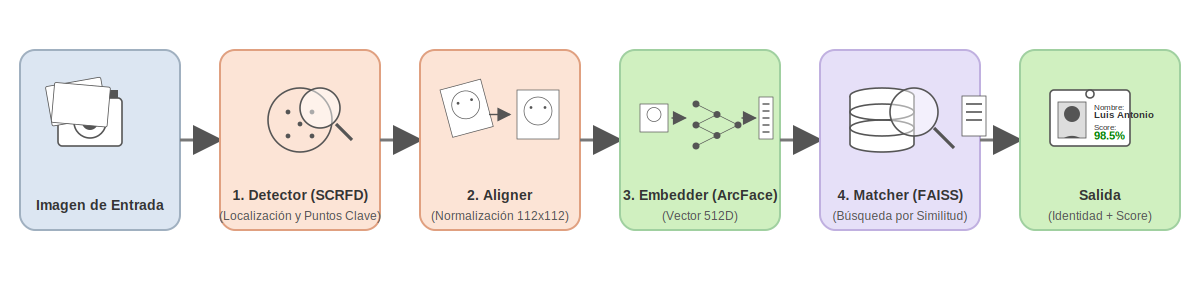
\includegraphics[width=0.95\textwidth]{arquitecture.pdf}
\caption{Flujo de datos a través de los componentes del sistema. Cada módulo procesa la salida del anterior hasta obtener la identidad de la persona.}
\label{fig:pipeline}
\end{figure}

Las interfaces principales se definen como protocolos de Python que especifican las firmas de los métodos requeridos:

\begin{lstlisting}[caption={Definición de interfaces del sistema}, label={lst:interfaces}]
@runtime_checkable
class Detector(Protocol):
    def detect(self, frame_bgr: np.ndarray) -> List[Detection]: ...

@runtime_checkable
class Aligner(Protocol):
    def align(self, frame_bgr: np.ndarray,
              kps_5pt: np.ndarray) -> np.ndarray: ...

@runtime_checkable
class Embedder(Protocol):
    def embed(self, face_bgr_112: np.ndarray) -> np.ndarray: ...

@runtime_checkable
class Matcher(Protocol):
    def add(self, label: str, embeddings: np.ndarray) -> None: ...
    def build(self) -> None: ...
    def search(self, embedding: np.ndarray,
               topk: int = 1) -> Tuple[List[str], List[float]]: ...
\end{lstlisting}

\subsection{Estructura del Proyecto}

El código se organiza en módulos con responsabilidades bien definidas:

\begin{verbatim}
metodos_final/
  app/
    core/           # Interfaces, configuración, utilidades
    backends/
      insightface/  # Implementación SCRFD + ArcFace + FAISS
      dlib/         # Implementación HOG/CNN + ResNet-34
    services/       # Servicios de enrollment y recognition
  scripts/          # CLIs para captura, indexado, inferencia
  models/           # Índices FAISS y archivos de labels
  data/             # Imágenes de enrollment
\end{verbatim}

La Figura \ref{fig:stack} presenta el stack tecnológico completo utilizado en el desarrollo del sistema, incluyendo las bibliotecas de análisis facial, búsqueda vectorial y herramientas de desarrollo.

\begin{figure}[H]
\centering
\includegraphics[width=0.95\textwidth]{stack.pdf}
\caption{Stack tecnológico del sistema. Se muestran los componentes de análisis facial (InsightFace, dlib, OpenCV), búsqueda vectorial (FAISS), base de desarrollo (Python, NumPy, uv) y hardware utilizado.}
\label{fig:stack}
\end{figure}

\subsection{Proceso de Enrolamiento}

El enrolamiento consiste en capturar múltiples imágenes faciales de cada persona que se desea reconocer, extraer sus embeddings y construir un índice de búsqueda. Los pasos son:

\begin{enumerate}
    \item \textbf{Captura}: Se activa la webcam y se detectan rostros frame a frame. Cuando se detecta exactamente un rostro con suficiente calidad (verificada mediante varianza del Laplaciano), se guarda la imagen alineada.
    \item \textbf{Extracción}: Para cada persona enrolada, se cargan sus imágenes alineadas y se extraen embeddings mediante el modelo ArcFace.
    \item \textbf{Indexación}: Se calcula el centroide (promedio normalizado) de los embeddings de cada persona y se construye el índice FAISS.
\end{enumerate}

La Figura \ref{fig:enrollment} muestra la interfaz de captura durante el proceso de enrolamiento. El sistema muestra una guía visual y el contador de imágenes capturadas.

\begin{figure}[H]
\centering
\includegraphics[width=0.7\textwidth]{enrollment_screenshot.png}
\caption{Interfaz de captura durante el proceso de enrolamiento. Se muestra la detección del rostro y el progreso de imágenes capturadas.}
\label{fig:enrollment}
\end{figure}

\subsection{Proceso de Reconocimiento}

Durante la inferencia, el sistema procesa cada frame de video ejecutando el pipeline completo:

\begin{enumerate}
    \item Detectar todos los rostros en el frame
    \item Para cada rostro detectado:
    \begin{enumerate}
        \item Alinear usando los landmarks de 5 puntos
        \item Extraer embedding de 512 dimensiones
        \item Buscar en el índice FAISS
        \item Comparar score con umbral de reconocimiento
    \end{enumerate}
    \item Dibujar cajas y etiquetas en el frame
    \item Mostrar resultado
\end{enumerate}

\subsection{Implementación del Backend InsightFace}

El backend principal utiliza los modelos de InsightFace. El detector SCRFD se inicializa mediante la clase FaceAnalysis:

\begin{lstlisting}[caption={Inicialización del detector SCRFD}, label={lst:scrfd}]
class SCRFDDetector:
    def __init__(self, config: Config, det_size=(640, 640)):
        self.app = FaceAnalysis(
            name=config.model_pack,
            allowed_modules=["detection"],
            providers=["CUDAExecutionProvider", "CPUExecutionProvider"]
            if config.ctx_id >= 0 else ["CPUExecutionProvider"],
        )
        self.app.prepare(ctx_id=config.ctx_id, det_size=det_size)

    def detect(self, frame_bgr: np.ndarray) -> List[Detection]:
        faces = self.app.get(frame_bgr)
        detections = []
        for face in faces:
            bbox = BBox(x1=int(face.bbox[0]), y1=int(face.bbox[1]),
                       x2=int(face.bbox[2]), y2=int(face.bbox[3]))
            detection = Detection(bbox=bbox, kps=face.kps,
                                 score=float(face.det_score))
            detections.append(detection)
        return detections
\end{lstlisting}

El embedder ArcFace extrae características del modelo de reconocimiento incluido en FaceAnalysis:

\begin{lstlisting}[caption={Extracción de embeddings con ArcFace}, label={lst:arcface}]
def embed(self, face_bgr_112: np.ndarray) -> np.ndarray:
    # Obtener modelo de reconocimiento
    rec_model = self.app.models["recognition"]

    # Convertir BGR a RGB
    face_rgb = face_bgr_112[:, :, ::-1]

    # Extraer embedding
    embedding = rec_model.get_feat(face_rgb).flatten()

    # Normalizar L2
    norm = np.linalg.norm(embedding)
    embedding = embedding / norm

    return embedding.astype(np.float32)
\end{lstlisting}

\subsection{Implementación del Backend dlib}

Como alternativa educativa, se implementó un backend basado en dlib y face\_recognition siguiendo el tutorial de PyImageSearch:

\begin{lstlisting}[caption={Detector y embedder con dlib}, label={lst:dlib}]
class DlibDetector:
    def detect(self, frame_bgr: np.ndarray) -> List[Detection]:
        frame_rgb = cv2.cvtColor(frame_bgr, cv2.COLOR_BGR2RGB)
        face_locations = face_recognition.face_locations(
            frame_rgb, model=self.model
        )
        detections = []
        for top, right, bottom, left in face_locations:
            bbox = BBox(x1=left, y1=top, x2=right, y2=bottom)
            detections.append(Detection(bbox=bbox, kps=None, score=0.99))
        return detections

class DlibEmbedder:
    def embed(self, face_bgr: np.ndarray) -> np.ndarray:
        face_rgb = cv2.cvtColor(face_bgr, cv2.COLOR_BGR2RGB)
        encodings = face_recognition.face_encodings(face_rgb)
        if not encodings:
            raise ValueError("No face found in image")
        return np.array(encodings[0], dtype=np.float32)
\end{lstlisting}

\section{Resultados y Discusión}

\subsection{Configuración Experimental}

Las pruebas se realizaron en un equipo con las siguientes características:
\begin{itemize}
    \item Procesador: Apple M2 Max (12 núcleos)
    \item Memoria RAM: 32 GB
    \item Sistema Operativo: macOS
    \item Python 3.12 con entorno virtual gestionado por uv
\end{itemize}

Se enrolaron 2 personas (LUIS y LESLY) con aproximadamente 15 imágenes cada una, capturadas mediante webcam en condiciones de iluminación interior típicas.

\subsection{Métricas de Rendimiento}

La Tabla \ref{tabla:rendimiento} presenta las métricas de rendimiento medidas durante las pruebas de reconocimiento en tiempo real.

\begin{table}[H]
\centering
\begin{tabular}{|l|c|c|}
\hline
\textbf{Métrica} & \textbf{InsightFace} & \textbf{dlib (HOG)} \\ \hline
FPS promedio & 12-15 & 18-22 \\ \hline
Tiempo detección (ms) & 45-60 & 25-35 \\ \hline
Tiempo embedding (ms) & 15-20 & 40-50 \\ \hline
Tiempo búsqueda (ms) & $<$1 & $<$1 \\ \hline
Dimensión embedding & 512 & 128 \\ \hline
\end{tabular}
\caption{Comparación de rendimiento entre backends}
\label{tabla:rendimiento}
\end{table}

La Figura \ref{fig:backends_tabla} presenta una comparación detallada de las características técnicas de ambos backends.

\begin{figure}[H]
\centering
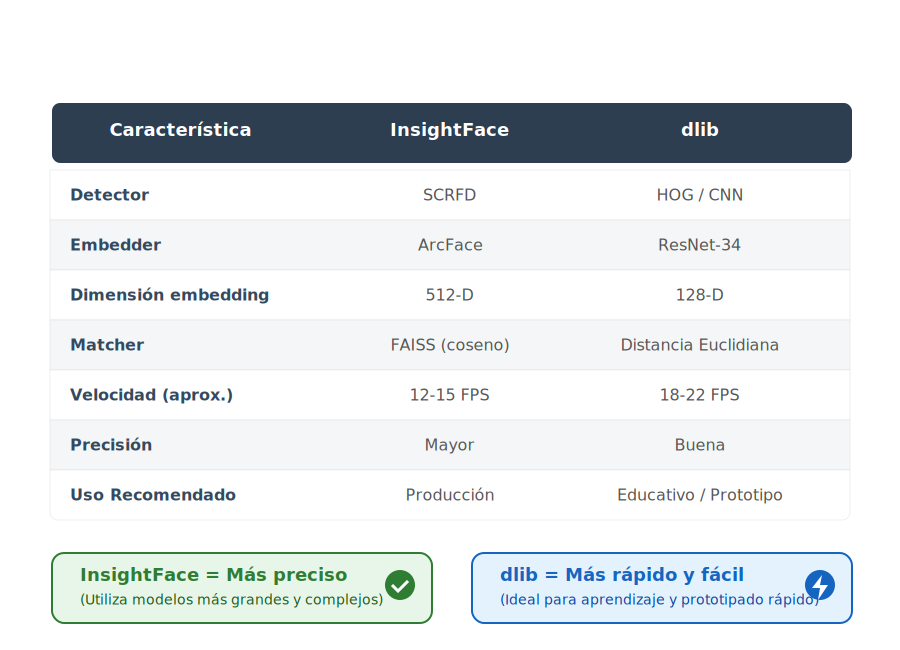
\includegraphics[width=0.95\textwidth]{backends.pdf}
\caption{Comparación técnica entre los backends InsightFace y dlib. Se detallan las diferencias en detector, embedder, dimensión de vectores, matcher y casos de uso recomendados.}
\label{fig:backends_tabla}
\end{figure}

El backend InsightFace presenta mayor tiempo de detección debido a la complejidad del modelo SCRFD, pero produce embeddings más rápidamente gracias a la optimización ONNX. El backend dlib con HOG es más rápido en detección pero más lento en la extracción de características.

\subsection{Precisión de Reconocimiento}

Se realizó una evaluación cuantitativa del sistema utilizando un conjunto de 26 imágenes de validación. La Figura \ref{fig:evaluacion} presenta los resultados obtenidos, incluyendo la matriz de confusión y el impacto del umbral de similitud.

\begin{figure}[H]
\centering
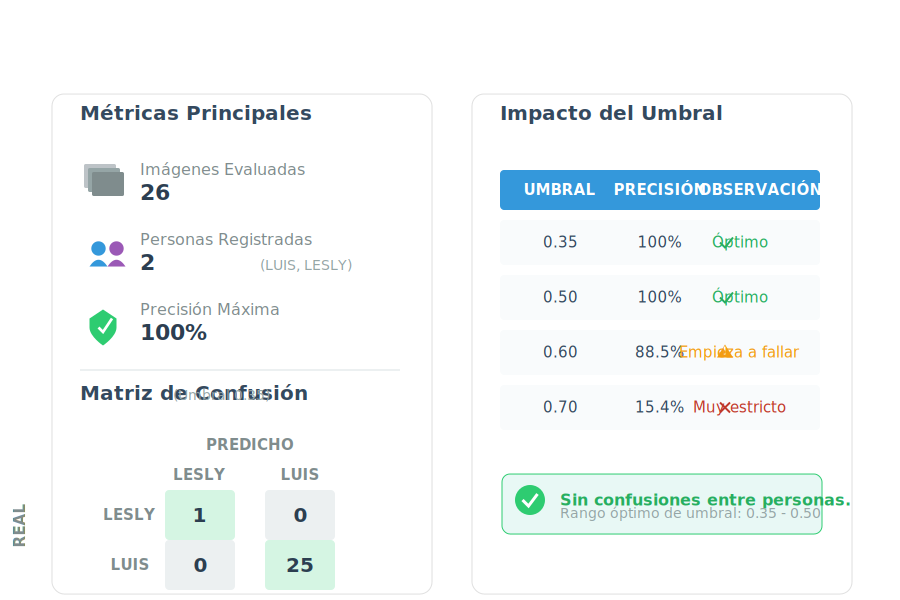
\includegraphics[width=0.95\textwidth]{eval.pdf}
\caption{Resultados de la evaluación del sistema. Izquierda: métricas principales y matriz de confusión con umbral 0.35. Derecha: impacto del umbral de similitud en la precisión.}
\label{fig:evaluacion}
\end{figure}

Los resultados demuestran que el sistema alcanza una precisión del 100\% con umbrales entre 0.35 y 0.50. La matriz de confusión muestra cero confusiones entre personas: todas las imágenes de LESLY fueron identificadas correctamente como LESLY, y todas las de LUIS como LUIS.

La Tabla \ref{tabla:umbral} resume el impacto del umbral de similitud:

\begin{table}[H]
\centering
\begin{tabular}{|c|c|l|}
\hline
\textbf{Umbral} & \textbf{Precisión} & \textbf{Observación} \\ \hline
0.35 & 100\% & Óptimo \\ \hline
0.50 & 100\% & Óptimo \\ \hline
0.60 & 88.5\% & Empieza a fallar \\ \hline
0.70 & 15.4\% & Muy estricto \\ \hline
\end{tabular}
\caption{Impacto del umbral de similitud en la precisión del sistema}
\label{tabla:umbral}
\end{table}

Un umbral demasiado alto (0.70) rechaza incluso a personas conocidas, clasificándolas como ``unknown''. El rango óptimo identificado es 0.35-0.50, donde el sistema reconoce correctamente sin generar falsos positivos.

\subsection{Análisis del Pipeline}

El servicio de reconocimiento integra los componentes de manera transparente:

\begin{lstlisting}[caption={Servicio de reconocimiento}, label={lst:service}]
class RecognitionService:
    def recognize(self, frame: np.ndarray) -> List[RecognitionResult]:
        # Detectar rostros
        detections = self.detector.detect(frame)

        results = []
        for detection in detections:
            # Alinear (solo InsightFace)
            if self.aligner and detection.kps is not None:
                face = self.aligner.align(frame, detection.kps)
            else:
                face = frame[detection.bbox.y1:detection.bbox.y2,
                            detection.bbox.x1:detection.bbox.x2]

            # Extraer embedding
            embedding = self.embedder.embed(face)

            # Buscar en indice
            labels, scores = self.matcher.search(embedding)

            # Aplicar umbral
            is_known = scores[0] >= self.threshold
            label = labels[0] if is_known else "unknown"

            results.append(RecognitionResult(
                bbox=detection.bbox,
                label=label,
                score=scores[0],
                is_known=is_known
            ))

        return results
\end{lstlisting}

\subsection{Visualización de Resultados}

El sistema dibuja cajas delimitadoras coloreadas (verde para conocidos, rojo para desconocidos) junto con la etiqueta y score de similitud. La Figura \ref{fig:resultado} ilustra un ejemplo típico de salida.

\begin{figure}[H]
\centering
\includegraphics[width=0.7\textwidth]{recognition_screenshot.png}
\caption{Ejemplo de salida del sistema de reconocimiento. Se muestra la caja delimitadora alrededor del rostro detectado, la etiqueta con la identidad y score de similitud, y el contador de FPS.}
\label{fig:resultado}
\end{figure}

\subsection{Discusión}

Los resultados obtenidos validan la efectividad de la arquitectura propuesta. La separación en componentes intercambiables permitió comparar fácilmente dos enfoques distintos (InsightFace vs dlib) sin modificar la lógica de alto nivel. Las Figuras \ref{fig:backend_insightface} y \ref{fig:backend_dlib} muestran una comparación visual del funcionamiento de ambos backends.

\begin{figure}[H]
\centering
\includegraphics[width=0.75\textwidth]{backend_insightface.png}
\caption{Reconocimiento facial con backend InsightFace (SCRFD + ArcFace). Se observa la detección del rostro con la identidad y score de similitud.}
\label{fig:backend_insightface}
\end{figure}

\begin{figure}[H]
\centering
\includegraphics[width=0.75\textwidth]{backend_dlib.png}
\caption{Reconocimiento facial con backend dlib (HOG + ResNet-34). Se muestra el mismo escenario procesado con el backend alternativo.}
\label{fig:backend_dlib}
\end{figure}

El modelo ArcFace demostró superior poder discriminativo, lo cual se atribuye a:
\begin{itemize}
    \item Mayor dimensionalidad del embedding (512 vs 128)
    \item Entrenamiento con margin angular que maximiza separabilidad
    \item Dataset de entrenamiento más grande y diverso
\end{itemize}

Por otro lado, el enfoque dlib resulta más accesible para propósitos educativos debido a su API simplificada y documentación extensa en tutoriales como los de PyImageSearch.

Las limitaciones identificadas incluyen:
\begin{itemize}
    \item Dependencia de la calidad de iluminación
    \item Dificultad con oclusiones parciales (mascarillas)
    \item Necesidad de re-enrollment si cambia significativamente la apariencia
\end{itemize}

\section{Conclusiones}

El presente trabajo cumplió satisfactoriamente los objetivos planteados. Se diseñó e implementó un sistema de reconocimiento facial funcional que opera en tiempo real, demostrando la aplicabilidad práctica de las técnicas de aprendizaje profundo estudiadas.

La arquitectura modular basada en interfaces demostró ser una decisión de diseño acertada. Permitió no solo comparar backends distintos, sino que además facilita futuras extensiones como la incorporación de detección de vida (anti-spoofing) o tracking de múltiples personas.

Los experimentos confirmaron que ArcFace produce embeddings más discriminativos que los métodos tradicionales basados en dlib, aunque ambos enfoques resultan viables para aplicaciones con conjuntos pequeños de identidades.

Como trabajo futuro se plantea:
\begin{itemize}
    \item Integrar un módulo de tracking para seguimiento temporal de personas
    \item Implementar detección de ataques de presentación (fotografías, videos)
    \item Exponer el sistema como API REST mediante FastAPI
\end{itemize}

El código fuente desarrollado queda disponible en el repositorio \url{https://github.com/lapillaga/face_recognition} como material de referencia para futuros estudiantes interesados en sistemas de visión por computador.


\newpage

\renewcommand\refname{Bibliografía}

\begin{thebibliography}{9}

\bibitem[De]{deng2019} J. Deng, J. Guo, N. Xue, and S. Zafeiriou. \textsl{ArcFace: Additive Angular Margin Loss for Deep Face Recognition}, IEEE/CVF Conference on Computer Vision and Pattern Recognition (CVPR), pp. 4690-4699, 2019. \url{https://arxiv.org/abs/1801.07698}

\bibitem[Gu]{guo2021} J. Guo, J. Deng, A. Lattas, and S. Zafeiriou. \textsl{Sample and Computation Redistribution for Efficient Face Detection}, International Conference on Learning Representations (ICLR), 2022. \url{https://arxiv.org/abs/2105.04714}

\bibitem[Jo]{johnson2019} J. Johnson, M. Douze, and H. Jégou. \textsl{Billion-scale similarity search with GPUs}, IEEE Transactions on Big Data, vol. 7, no. 3, pp. 535-547, 2019. \url{https://arxiv.org/abs/1702.08734}

\bibitem[Ki]{king2017} D. E. King. \textsl{High Quality Face Recognition with Deep Metric Learning}, dlib blog, 2017. \url{http://blog.dlib.net/2017/02/high-quality-face-recognition-with-deep.html}

\bibitem[Wa]{wang2021} M. Wang and W. Deng. \textsl{Deep Face Recognition: A Survey}, Neurocomputing, vol. 429, pp. 215-244, 2021. \url{https://arxiv.org/abs/1804.06655}

\bibitem[In]{insightface} J. Guo and J. Deng. \textsl{InsightFace: State-of-the-art 2D and 3D Face Analysis Project}, GitHub repository, 2024. \url{https://github.com/deepinsight/insightface}



\end{thebibliography}


\newpage

\section*{Anexos}

\subsection*{A. Instrucciones de Instalación}

El proyecto utiliza \texttt{uv} para gestión de dependencias:

\begin{verbatim}
# Clonar repositorio
git clone <repo_url>
cd metodos_final

# Crear entorno virtual e instalar dependencias
uv sync

# Configurar variables de entorno
cp .env.example .env
# Editar .env según sea necesario
\end{verbatim}

\subsection*{B. Comandos de Ejecución}

\begin{verbatim}
# Capturar imágenes de enrollment
python scripts/insightface/01_capture_enroll.py --name LUIS --num 15

# Construir índice FAISS
python scripts/insightface/02_build_index.py

# Ejecutar reconocimiento por webcam
python scripts/insightface/03_run_webcam.py --threshold 0.35

# Ejecutar con backend dlib
python scripts/dlib/02_run_webcam.py --detector-model hog
\end{verbatim}

\subsection*{C. Variables de Configuración}

\begin{verbatim}
# .env
CTX_ID=-1        # -1=CPU, 0=GPU
THRESH=0.35      # Umbral de reconocimiento
CAMERA_ID=0      # ID de cámara
DISPLAY=1        # 1=mostrar ventana, 0=headless
MODEL_PACK=buffalo_l  # Modelo InsightFace
\end{verbatim}


\end{document}
